\section{Process Management}\label{sec:Process_Management}
\begin{definition}[Process]\label{def:Process}
  A \emph{process} is a \nameref{def:Program} in the midst of execution, and all its related resources.
  In fact, two or more processes can exist that are executing the same program.
  Processes are, however, more than just the executing program code (often called the text section in Unix).
  They also include a set of resources such as open files and pending signals, internal \nameref{def:Kernel} data, processor state, a memory address space with one or more memory mappings, one or more \nameref{def:Thread}s of execution, and a data section containing global variables.

  Processes, in effect, are the living result of running program code.
\end{definition}

\begin{definition}[Program]\label{def:Program}
  A \emph{program} is object code stored on some media, typically as a \nameref{def:File}.
  These contain the instructions that the processor will execute when the program is running as a \nameref{def:Process}.
  These instructions are stored in what is called the \emph{text section} of the program.
  It also contains statically allocated information, such as \kernelinline{static} variables.
\end{definition}

Occassionally, \nameref{def:Thread}s can be subject to \nameref{def:Preemption}.

\begin{definition}[Preemption]\label{def:Preemption}
  \emph{Preemption} is the act of temporarily interrupting a task being carried out by a computer system, without requiring its cooperation, and with the intention of resuming the task at a later time.
  Such changes of the executed task are known as context switches.
  It is normally carried out by a privileged task or part of the system known as a preemptive scheduler, which has the power to preempt, or interrupt, and later resume, other tasks in the system.

  In any given system design, some operations performed by the system may not be preemptible.
  This usually applies to \nameref{def:Kernel} functions and service interrupts which, if not permitted to run to completion, would tend to produce race conditions resulting in deadlock.
\end{definition}

On modern \nameref{def:Operating_System}s, \nameref{def:Process}es provide two virtualizations:
\begin{enumerate}[noitemsep]
\item a virtualized processor
  \begin{itemize}[noitemsep]
  \item The virtual processor gives \emph{this} \nameref{def:Process} the illusion that it alone monopolizes the system, despite possibly sharing the processor among hundreds of other processes.
\end{itemize}
\item Virtual memory lets the process allocate and manage memory as if it alone owned all the memory in the system.
  \begin{itemize}[noitemsep]
  \item \nameref{def:Thread}s share the virtual memory abstraction, whereas each receives its own virtualized processor.
  \end{itemize}
\end{enumerate}

\subsection{The Process Life Cycle}\label{subsec:Process_Life_Cycle}
A \nameref{def:Process} begins its life when, the \kernelinline{fork()} \nameref{def:System_Call} is called.
This creates a new \nameref{def:Process} by duplicating an existing one.
The \nameref{def:Process} that calls \kernelinline{fork()} is the \textbf{parent}, whereas the new \nameref{def:Process} is the \textbf{child}.
The \kernelinline{fork()} \nameref{def:System_Call} returns from the kernel twice: once in the \textbf{parent} and once in the newborn \textbf{child}.
The parent resumes execution and the child starts execution at the same place, where the call to \kernelinline{fork()} returns.

Often, immediately after a \texttt{fork} it is desirable to execute a new, different \nameref{def:Program}.
The \kernelinline{exec()} family of function calls creates a new address space and loads a new program into it.

Finally, a program exits via the \kernelinline{exit()} \nameref{def:System_Call}.
This function terminates the \nameref{def:Process} and frees all its resources.
A parent \nameref{def:Process} can inquire about the status of a terminated child via the \kernelinline{wait4()} \nameref{def:System_Call}, which enables a \nameref{def:Process} to wait for the termination of a specific \nameref{def:Process}.
When a \nameref{def:Process} exits, it is placed into a special zombie state that represents terminated \nameref{def:Process}es until the parent calls \kernelinline{wait()} or \kernelinline{waitpid()}.

\subsubsection{Process States}\label{subsubsec:Process_States}
Every \nameref{def:Process} exists in a state that describes how the process can and will behave.
\begin{itemize}[noitemsep]
\item \textbf{New}: The process is in the stage of being created.
\item \textbf{Ready}: The process has all the resources available that it needs to run, but the CPU is not currently working on this process's instructions.
\item \textbf{Running}: The CPU is working on this process's instructions.
\item \textbf{Waiting}: The process cannot run at the moment, because it is waiting for some resource to become available or for some event to occur.
\item \textbf{Terminated}: The process has completed.
\end{itemize}

\begin{figure}[h!tbp]
  \centering
  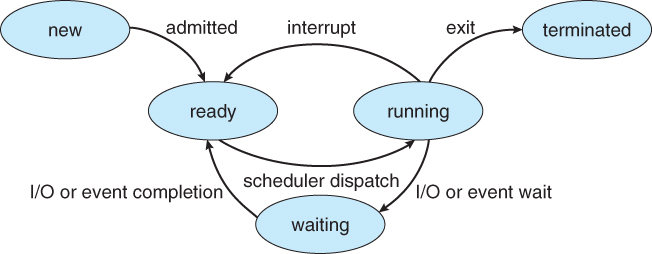
\includegraphics[scale=0.85]{./Process_Life_Cycle.jpg}
  \caption{Process Life Cycle}
  \label{fig:Process_Life_Cycle}
\end{figure}

\subsubsection{Process Control Blocks and Context Switching}\label{subsubsec:PCBs_Context_Switching}
The information that is saved during a \nameref{def:Context_Switch} (An example is shown in \Cref{fig:Context_Switch}) is saved in the \nameref{def:Process_Control_Block}.

\begin{definition}[Context Switch]\label{def:Context_Switch}
  A \emph{context switch} is performed when a computer is performing several different \nameref{def:Process}es in sequence.
  A context switch involves saving the state of the currently running \nameref{def:Process} into a \nameref{def:Process_Control_Block}, and then loading a waiting process from its \nameref{def:Process_Control_Block}.
  After saving the information, every register in the CPU has its values changes to the new control blocks values, and the CPU continues execution.

  A visualization of a context switch is shown in \Cref{fig:Context_Switch}.
\end{definition}

\begin{figure}[h!tbp]
  \centering
  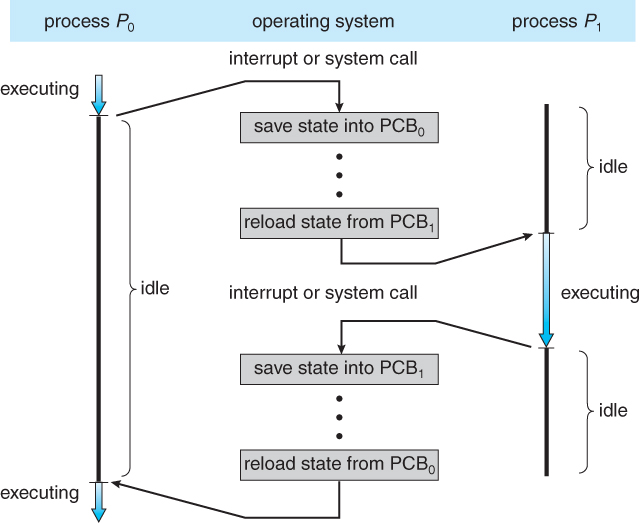
\includegraphics[scale=0.85]{./Context_Switch.jpg}
  \caption{Diagram of a Context Switch}
  \label{fig:Context_Switch}
\end{figure}

\begin{definition}[Process Control Block]\label{def:Process_Control_Block}
  The \emph{process control block} (\emph{PCB}) contains \textbf{ALL} the state information (the processor's context) needed for a CPU to perform a context switch, either because of \nameref{def:Preemption} or because the process terminated.
  The information that the PCB contains includes:
  \begin{itemize}[noitemsep]
  \item Process State: Running, waiting, etc., as discussed in \Cref{subsubsec:Process_States}
  \item Process ID (PID), and parent process ID (PPID).\@
  \item CPU registers and Program Counter: Saved and restored when swapping processes in and out of the CPU.\@
  \item CPU-Scheduling information: Priority information and pointers to scheduling queues.
  \item Memory-Management information: Page tables or segment tables.
  \item Accounting information: \nameref{def:User} and \nameref{def:Kernel} CPU time consumed, account numbers, limits, etc.
  \item I/O Status information: Devices allocated, open file tables, etc.
  \end{itemize}
\end{definition}

\begin{figure}[h!tbp]
  \centering
  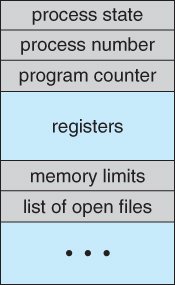
\includegraphics[scale=0.85]{./Process_Control_Block.jpg}
  \caption{Process Control Block}
  \label{fig:Process_Control_Block}
  \begin{remark*}
    In \Cref{fig:Process_Control_Block}, the Process Number field is the PID of the \nameref{def:Process}.
  \end{remark*}
\end{figure}

The time spent performing a context-switch is pure overhead, because the system does no useful work while switching.
Switching speed varies from machine to machine, depending on the memory speed, the number of registers that must be copied, and the existence of special instructions (a single instruction to load or store all registers).
A typical speed is a few milliseconds.
Context-switch times are also highly dependent on hardware support.

The more complex the operating system, the greater the amount of work that must be done during a context switch.
In addition, advanced memory-management techniques may require that extra data be switched with each context.
For instance, the address space of the current process must be preserved as the space of the next task is prepared for use.

%%% Local Variables:
%%% mode: latex
%%% TeX-master: "../../EDAF35-Operating_Systems-Reference_Sheet"
%%% End:


\subsection{Process Creation}\label{subsec:Process_Creation}
Most operating systems implement a \texttt{spawn} mechanism to create a new process in a new address space, read in an executable, and begin executing it.
UNIX takes the unusual approach of separating these steps into two distinct functions: \kernelinline{fork()} and \kernelinline{exec()}.
The first, \kernelinline{fork()}, creates a child process that is a copy of the current task.
It differs from the parent only in:
\begin{itemize}[noitemsep]
\item Its PID (which is unique)
\item Its PPID (parent’s PID, which is set to the original process)
\item Certain resources and statistics, such as pending signals, which are not inherited
\end{itemize}

The second function, \kernelinline{exec()}, loads a new executable into the address space and begins executing it.

\subsubsection{Copy-on-Write}\label{subsubsec:Process_Copy_on_Write}
In Linux, \kernelinline{fork()} is implemented through the use of copy-on-write pages.
Copy-on-write (or CoW) is a technique to delay or altogether prevent copying of the data.
Rather than duplicate the process address space, the parent and the child can share a single read-only copy.

The data, however, is marked in such a way that if it is written to, a duplicate is made and each \nameref{def:Process} receives their own unique copy.
Consequently, the duplication of resources occurs only when they are written; until then, they are shared read-only.
This technique delays the copying of each page in the address space until it is actually written to.
In the case that the pages are never written—for example, if \kernelinline{exec()} is called immediately after \kernelinline{fork()}—they never need to be copied.

The only overhead incurred by \kernelinline{fork()} is the duplication of the parent’s page tables and the creation of a unique \nameref{def:Process_Descriptor} for the child.
In the common case that a \nameref{def:Process} executes a new executable image immediately after forking, this optimization prevents the wasted copying of large amounts of data.

\subsubsection{Forking}\label{subsubsec:Forking}
The bulk of the work in forking is handled by \kernelinline{do_fork()}, which is defined in \kernelinline{kernel/fork.c}, by calling \kernelinline{copy_process()} and then starting the process.
The interesting work is done by \kernelinline{copy_process()}:
\begin{enumerate}
\item It calls \kernelinline{dup_task_struct()}, which creates a new kernel stack, \kernelinline{thread_info} structure, and \kernelinline{task_struct} for the new process.
  The new values are identical to those of the current task.
  At this point, the child and parent \nameref{def:Process_Descriptor}s are identical.
\item It then checks that the new child will not exceed the resource limits on the number of processes for the current user.
\item The child needs to differentiate itself from its parent.
  Various members of the \nameref{def:Process_Descriptor} are cleared or set to initial values.
  Members of the \nameref{def:Process_Descriptor} not inherited are primarily statistical information.
  The bulk of the values in \kernelinline{task_struct} remain unchanged.
\item The child’s state is set to \kernelinline{TASK_UNINTERRUPTIBLE} to ensure that it does not yet run.
\item \kernelinline{copy_process()} calls \kernelinline{copy_flags()} to update the flags member of the \kernelinline{task_struct}.
  The \kernelinline{PF_SUPERPRIV} flag, which denotes whether a task used superuser privileges, is cleared.
  The \kernelinline{PF_FORKNOEXEC} flag, which denotes a process that has not called \kernelinline{exec()}, is set.
\item It calls \kernelinline{alloc_pid()} to assign an available PID to the new task.
\item Depending on the flags passed to \kernelinline{clone()}, \kernelinline{copy_process()} either duplicates or shares open \nameref{def:File}s, filesystem information, signal handlers, process address space, and namespace.
  These resources are typically shared between \nameref{def:Thread}s in a given \nameref{def:Process}; otherwise they are unique and copied here.
\item Finally, \kernelinline{copy_process()} cleans up and returns to the caller a pointer to the new child.
\end{enumerate}

Back in \kernelinline{do_fork()}, if \kernelinline{copy_process()} returns successfully, the new child is woken up and run.
Deliberately, the kernel runs the child process first.

\kernelinline{fork()} returns \texttt{0} in the newly created child process, and the PID of the child in the parent.
Then, \kernelinline{exec()} \textbf{COMPLETELY REPLACES THE PROCESS' MEMORY}, meaning that after an \kernelinline{exec()}, the child is not executing the same program anymore.

%%% Local Variables:
%%% mode: latex
%%% TeX-master: "../../EDAF35-Operating_Systems-Reference_Sheet"
%%% End:


\subsection{Process Scheduling}\label{subsec:Process_Scheduling}
With multiprogramming, the objective is to have \textbf{some} \nameref{def:Process} running at all times.
Note that we are discussing a computer with a single CPU, and likely a single \nameref{def:Thread} here.
Time sharing makes the CPU \nameref{def:Context_Switch} so frequently that users can interact with each program and it seems like they are all running concurrently.

\begin{definition}[Process Scheduler]\label{def:Process_Scheduler}
  The \emph{process scheduler} is responsible for selecting an available process (one in the New, Ready, or Running states discussed in \Cref{subsubsec:Process_States}) from one of possibly many queues to run next.
\end{definition}

\subsubsection{Scheduling Queues}\label{subsubsec:Scheduling_Queues}
When a \nameref{def:Process} enters the system, it is put in the \textbf{Job Queue}, which consists of \textbf{EVERY} process on the system.

The processes that are in main memory, are ready, and waiting to execute are in the \textbf{Ready Queue}.
The \nameref{def:Process_Control_Block}s are kept in a doubly linked list, with the first and last PCBs explicitly marked by the list itself and a pointer to the next PCB in the ready queue in each PCB.\@

There are other queues as well:
\begin{itemize}[noitemsep]
\item \textbf{Device Queue}: Completion of I/O Request(s)
  \begin{itemize}[noitemsep]
  \item Each device has its own queue.
  \end{itemize}
\end{itemize}

These various queues can be represented by \Cref{fig:Queues}.
\begin{figure}[h!tbp]
  \centering
  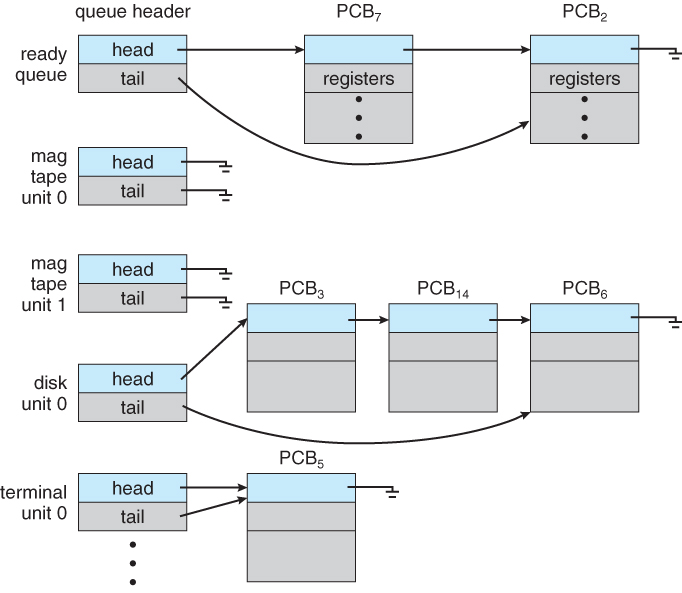
\includegraphics[scale=1.00]{./Queues.jpg}
  \caption{Various System Queues}
  \label{fig:Queues}
\end{figure}

A good visualization of how \nameref{def:Process}es and their queues work is shown in \Cref{fig:Queuing_Diagram}.

\begin{figure}[h!tbp]
  \centering
  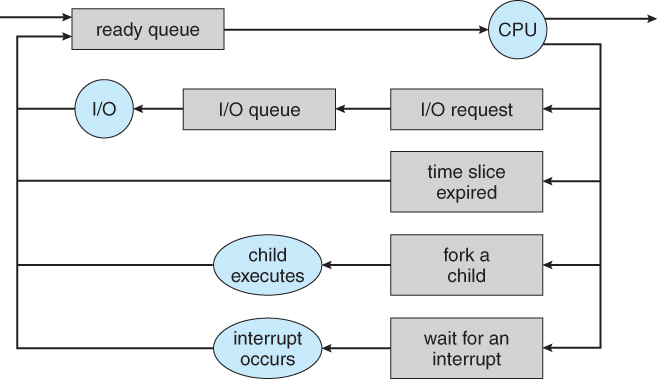
\includegraphics[scale=1.00]{./Queuing_Diagram.jpg}
  \caption{Queuing Diagram for Process Scheduling}
  \label{fig:Queuing_Diagram}
\end{figure}

\subsubsection{Schedulers}\label{subsubsec:Schedulers}
\begin{definition}[Scheduler]\label{def:Scheduler}
  A \emph{scheduler} is responsible for selecting the \nameref{def:Process} from one of the queues to execute next.
\end{definition}

Typically, many more \nameref{def:Process}es are submitted at once than can be handled immediately.
So, some are sent to a mass-storage device where they are keyp for later scheduling by the \emph{long-term scheduler} or \emph{job scheduler}.
The \emph{short-term scheduler}, or the \emph{CPU scheduler} selects from the \nameref{def:Process}es that are ready to execute and allocates the CPU to them.
The CPU scheduler is run every hundred milliseconds, whereas the job scheduler may be run every few minutes.
This allows the job scheduler to run for longer periods of time, because it is active for less time overall.

The job scheduler determines the \emph{degree of multiprogramming}, by determining how many \nameref{def:Process}es can live in memory at any given time.
If the degree of multiprogramming is stable, then the average rate of process creation must be equal to the average departure rate of processes leaving the system.
Most desktop \nameref{def:Operating_System}s do not use the long-term scheduler.
Instead they put all tasks into the short-term queue, and rely on human behavior to help control the business of the systems.

\begin{definition}[I/O Bound]\label{def:IO_Bound}
  An \emph{I/O Bound} \nameref{def:Process} is one where most of the process's time is spent performing I/O rather than computations.
\end{definition}

\begin{definition}[CPU-Bound]\label{def:CPU_Bound}
  A \emph{CPU-Bound} \nameref{def:Process} spends most of its time performing computations.
\end{definition}

It is important to have a good mix of \nameref{def:IO_Bound} and \nameref{def:CPU_Bound} processes, so that no single queue is ever too full, improving overall system throughput.

There are also \emph{medium-term scheduler}s that perform \emph{swapping}.
This scheduler removes a \nameref{def:Process} from memory, store it somewhere, then reintroduce the process to memory again later.

%%% Local Variables:
%%% mode: latex
%%% TeX-master: "../../EDAF35-Operating_Systems-Reference_Sheet"
%%% End:


\subsection{The Process Descriptor and Task \texttt{struct}}\label{subsec:Process_Descriptor_Task_Struct}
\begin{definition}[Task List]\label{def:Task_List}
  The \nameref{def:Kernel} stores the list of \nameref{def:Process}es in a circular doubly-linked list called the \emph{task list}.
  Each element in the task list is a \nameref{def:Process_Descriptor} of the type \kernelinline{struct task_struct}.
\end{definition}

\begin{definition}[Process Descriptor]\label{def:Process_Descriptor}
  The \emph{process descriptor} contains all the information about a specific \nameref{def:Process}, including:
  \begin{itemize}[noitemsep]
  \item Open files
  \item The \nameref{def:Process}’s address space,
  \item Pending signals,
  \item The \nameref{def:Process}’s state,
  \item The \nameref{def:Process}'s priority
  \item The \nameref{def:Process}'s policy
  \item The \nameref{def:Process}'s parent
  \item The \nameref{def:Process}'s id (PID)
  \end{itemize}

  In Linux, the process descriptor is of type \kernelinline{struct task_struct}, which is defined in \texttt{<linux/sched.h>}.
\end{definition}

\subsubsection{Allocating the Process Descriptor}\label{subsubsec:Allocate_Process_Descriptor}
Like in any other programming language, the \kernelinline{task_struct} record must be initialized somehow.
This is done with the \emph{slab allocator} to provide object reuse and \nameref{def:Cache_Coloring}.

\begin{definition}[Cache Coloring]\label{def:Cache_Coloring}
  \emph{Cache coloring} (also known as page coloring) is the process of attempting to allocate free pages that are contiguous from the CPU cache's point of view, in order to maximize the total number of pages cached by the processor.
  Cache coloring is typically employed by low-level dynamic memory allocation code in the operating system, when mapping virtual memory to physical memory.
  A virtual memory subsystem that lacks cache coloring is less deterministic with regards to cache performance, as differences in page allocation from one program run to the next can lead to large differences in program performance.
\end{definition}

\subsubsection{Storing the Process Descriptor}\label{subsubsec:Storing_Process_Descriptor}
The system identifies \nameref{def:Process}es by a unique Process Identification Value or PID.\@
The PID is a numerical value represented by the opaque type\footnote{``An opaque type is a data type whose physical representation is unknown or irrelevant''~\cite[pg.~26]{LKD3}.} \kernelinline{pid_t}, which is typically an \kernelinline{int}.
Because of backward compatibility with earlier \textsc{unix} and Linux versions, the default maximum value is only 32,768 (that of a \kernelinline{(short int)}), although the value can be increased as high as four million (this is controlled in \kernelinline{<linux/threads.h>}).
The \nameref{def:Kernel} stores this value as PID inside each \nameref{def:Process_Descriptor}.
This maximum value is important because it is essentially the maximum number of \nameref{def:Process}es that may exist concurrently on the system.

Inside the \nameref{def:Kernel}, tasks are typically referenced directly by a pointer to their \kernelinline{task_struct} structure.
In fact, most \nameref{def:Kernel} code that deals with \nameref{def:Process}es works directly with \kernelinline{struct task_struct}.
Consequently, it is useful to be able to quickly look up the \nameref{def:Process_Descriptor} of the currently executing task, which is done via the current macro.
This macro must be independently implemented by each architecture.
Some architectures save a pointer to the \kernelinline{task_struct} structure of the currently running \nameref{def:Process} in a register, enabling for efficient access.
Other architectures make use of the fact that \kernelinline{struct thread_info} is stored on the \nameref{def:Kernel} stack to calculate the location of \kernelinline{thread_info} and subsequently the \kernelinline{task_struct}.

\subsubsection{Process State}\label{subsubsec:Process_State}
The state field of the process descriptor describes the current condition of the process.
Each process on the system is in exactly one of five different states.
This value is represented by one of five flags:
\begin{enumerate}[noitemsep]
\item \kernelinline{TASK_RUNNING}: The process is runnable; it is either currently running or on a runqueue waiting to run.
  This is the only possible state for a \nameref{def:Process} executing in \nameref{def:User}-space; it can also apply to a process in \nameref{def:Kernel}-space that is actively running.
\item \kernelinline{TASK_INTERRUPTIBLE}: The \nameref{def:Process} is sleeping (that is, it is blocked), waiting for some condition to exist.
  When this condition exists, the \nameref{def:Kernel} sets the \nameref{def:Process}’s state to \kernelinline{TASK_RUNNING}.
  The \nameref{def:Process} also awakes prematurely and becomes runnable if it receives a signal.
\item \kernelinline{TASK_UNINTERRUPTIBLE}: This state is identical to \kernelinline{TASK_INTERRUPTIBLE} \textbf{except that it does not wake up and become runnable if it receives a signal}.
  This is used in situations where the \nameref{def:Process} must wait without interruption or when the event is expected to occur quite quickly.
  Because the task does not respond to signals in this state, \kernelinline{TASK_UNINTERRUPTIBLE} is less often used than \kernelinline{TASK_INTERRUPTIBLE}.
\item \kernelinline{__TASK_TRACED}: The \nameref{def:Process} is being traced by another \nameref{def:Process}, such as a debugger, via \texttt{ptrace}.
\item \kernelinline{__TASK_STOPPED}: \nameref{def:Process} execution has stopped; the task is not running nor is it eligible to run.
  This occurs if the task receives the \texttt{SIGSTOP}, \texttt{SIGTSTP}, \texttt{SIGTTIN}, or \texttt{SIGTTOU} signal or if it receives any signal while it is being debugged.
\end{enumerate}

\subsubsection{Manipulating the Current Process's State}\label{subsubsec:Manipulate_Current_Process_State}
Kernel code often needs to change a process’s state.
The preferred mechanism is using
\begin{minted}[frame=lines,linenos]{c}
set_task_state(task, state); /* set task ‘task’ to state ‘state’ */
\end{minted}

This function sets the given \texttt{task} to the given \texttt{state}.
If applicable, it also provides a memory barrier to force ordering on other processors.
This is only needed on SMP systems.

\subsubsection{Process Context}\label{subsubsec:Process_Context}
Normal program execution occurs in \nameref{def:User}-space.
When a program executes a system call or triggers an exception, it enters \nameref{def:Kernel}-space.
At this point, the \nameref{def:Kernel} is said to be ``executing on behalf of the process'' and is in \nameref{def:Process}-context.
When in process context, the \texttt{current} macro is valid.

\begin{remark*}
  Other than process context there is \nameref{def:Interrupt}-context.
  In interrupt context, the system is not running on behalf of a process but is executing an interrupt handler.
  No \nameref{def:Process} is tied to interrupt handlers.
\end{remark*}

Upon exiting the kernel, the \nameref{def:Process} resumes execution in \nameref{def:User}-space, unless a higher-priority process has become runnable in the interim.
If that happens, the scheduler is invoked to select the higher priority process.
\nameref{def:System_Call}s and exception handlers are well-defined interfaces into the kernel.
A \nameref{def:Process} can begin executing in kernel-space only through one of these interfaces.
All access to the \nameref{def:Kernel} is through these interfaces.

\subsubsection{Process Family Tree}\label{subsubsec:Process_Family_Tree}
All processes are descendants of the init \nameref{def:Process}, whose PID is one.
The kernel starts \texttt{init} in the last step of the boot process.
The \texttt{init} process, in turn, reads the system initscripts and executes more programs, eventually completing the boot process.

Every process on the system has exactly one parent.
Likewise, every process has zero or more children.
Processes that are all direct children of the same parent are called siblings.
The relationship between processes is stored in the process descriptor.
Each \kernelinline{task_struct} has a pointer to the parent’s \kernelinline{task_struct}, named \texttt{parent}, and a list of children, named \texttt{children}.

%%% Local Variables:
%%% mode: latex
%%% TeX-master: "../../EDAF35-Operating_Systems-Reference_Sheet"
%%% End:


\subsection{Process Termination}\label{subsec:Process_Termination}
When a process terminates, the \nameref{def:Kernel} releases the resources owned by the process and notifies the child’s parent of its demise.
Usually, process destruction is self-induced.
It occurs when the process calls the \kernelinline{exit()} \nameref{def:System_Call}.
This can be done either explicitly when it is ready to terminate or implicitly on return from the main subroutine of any program (The C compiler places a call to \kernelinline{exit()} after \kernelinline{main()} returns).

A process can also terminate involuntarily.
This occurs when the process receives a signal or exception it cannot handle or ignore.

Regardless of how a process terminates, the bulk of the work is handled by \kernelinline{do_exit()}, defined in \kernelinline{kernel/exit.c}, which completes a number of chores:
\begin{enumerate}
\item It sets the \kernelinline{PF_EXITING} flag in the flags member of the \kernelinline{task_struct}.
\item It calls \kernelinline{del_timer_sync()} to remove any kernel timers.
  Upon return, it is guaranteed that no timer is queued and that no timer handler is running.
\item If BSD process accounting is enabled, \kernelinline{do_exit()} calls \kernelinline{acct_update_integrals()} to write out accounting information.
\item It calls \kernelinline{exit_mm()} to release the \kernelinline{mm_struct} held by this process.
  If no other process is using this address space, i.e.\ the address space is not shared, the \nameref{def:Kernel} then destroys it.
\item It calls \kernelinline{exit_sem()}.
  If the process is queued waiting for an IPC semaphore, it is dequeued here.
\item It then calls \kernelinline{exit_files()} and \kernelinline{exit_fs()} to decrement the usage count of objects related to file descriptors and filesystem data, respectively.
  If either usage counts reach zero, the object is no longer in use by any process, and it is destroyed.
\item It sets the \nameref{def:Process}’s exit code, stored in the \kernelinline{exit_code} member of the \kernelinline{task_struct}, to the code provided by \kernelinline{exit()} or whatever \nameref{def:Kernel} mechanism forced the termination.
  The exit code is stored here for optional retrieval by the parent.
\item It calls \kernelinline{exit_notify()} to send signals to the \nameref{def:Process}’s parent, reparents any of the \nameref{def:Process}’s children to another thread in their thread group or the init process, and sets the \nameref{def:Process}’s exit state, stored in \kernelinline{exit_state} in the \kernelinline{task_struct} structure, to \kernelinline{EXIT_ZOMBIE}.
\item \kernelinline{do_exit()} calls \kernelinline{schedule()} to switch to a new process.
  Because the process is now not schedulable, this is the last code the \nameref{def:Process} will ever execute.
  \kernelinline{do_exit()} never returns.
\end{enumerate}

At this point, we have a \nameref{def:Zombie_Process}.

\begin{definition}[Zombie Process]\label{def:Zombie_Process}
  A \emph{zombie process} in Linux is a process that has been completed, but its entry still remains in the process table due to lack of correspondence between the parent and child \nameref{def:Process}es.
  This happens when the \nameref{def:Process} has been terminated, but the \nameref{def:Process_Descriptor} has \textbf{not} be deallocated yet.

  \begin{itemize}[noitemsep]
  \item All objects associated with the \nameref{def:Process} are freed.
    \begin{itemize}[noitemsep]
    \item This assumes that this \nameref{def:Process} was the only one using these objects, i.e.\ no other \nameref{def:Thread}s/\nameref{def:Process}es were using them.
    \end{itemize}
  \item The \nameref{def:Process} is not runnable and no longer has an address space in which to run.
  \item The process is in the \kernelinline{EXIT_ZOMBIE} exit state.
  \item The only memory it occupies is its \nameref{def:Kernel} stack, the \kernelinline{thread_info} structure, and the \kernelinline{task_struct} structure.
  \item The \nameref{def:Process} exists solely to provide information to its parent.
    After the parent retrieves the information, or notifies the \nameref{def:Kernel} that it is uninterested, the remaining memory held by the process is freed and returned to the system for use.
  \end{itemize}
\end{definition}

\subsubsection{Removing a Process Descriptor}\label{subsubsec:Remove_Process_Descriptor}
After \kernelinline{do_exit()} completes, the \nameref{def:Process_Descriptor} for the terminated \nameref{def:Process} still exists, but the \nameref{def:Process} is a \nameref{def:Zombie_Process} and is unable to run.
By remaining a \nameref{def:Process}, albeit a \nameref{def:Zombie_Process}, this enables the system to obtain information about a child \nameref{def:Process} after it has terminated.

\begin{center}
  \large{\textbf{Consequently, the acts of cleaning up after a \nameref{def:Process} and removing its \nameref{def:Process_Descriptor} are separate.}}
\end{center}

\textbf{After} the parent has obtained information on its terminated child, or signified to the \nameref{def:Kernel} that it does not care, the child’s \kernelinline{task_struct} is deallocated.
The \kernelinline{wait()} family of functions are implemented via a single \nameref{def:System_Call}, \kernelinline{wait4()}.
The standard behavior is to suspend execution of the calling task until one of its children exits, at which time the function returns with the PID of the exited child.
Additionally, a pointer is provided to the function that on return holds the exit code of the terminated child.

When it is time to finally deallocate the \nameref{def:Process_Descriptor}, \kernelinline{release_task()} is invoked.
It does the following:
\begin{enumerate}
\item Calls \kernelinline{__exit_signal()}, which calls \kernelinline{__unhash_process()}, which in turns calls \kernelinline{detach_pid()} to remove the process from the PIDhash and remove the process from the task list.
\item \kernelinline{__exit_signal()} releases any remaining resources used by the now dead process and finalizes statistics and bookkeeping.
\item If the task was the last member of a thread group, and the leader is a zombie, then \kernelinline{release_task()} notifies the zombie leader’s parent.
\item \kernelinline{release_task()} calls \kernelinline{put_task_struct()} to free the pages containing the \nameref{def:Process}’s \nameref{def:Kernel} stack and \kernelinline{thread_info} structure and deallocate the slab cache containing the \kernelinline{task_struct}.
\end{enumerate}

At this point, the \nameref{def:Process_Descriptor} and all resources belonging solely to the process
have been freed.

\subsubsection{Parentless Tasks}\label{subsubsec:Parentless_Tasks}
If a parent exits before its children, some mechanism must exist to reparent any child tasks to a new process, or else parentless terminated processes would forever remain \nameref{def:Zombie_Process}es, wasting system memory.
The solution is to reparent a task’s children on exit to either another \nameref{def:Process} in the current \nameref{def:Thread} group or, if that fails, the \texttt{init} process.

When a suitable parent for the child(ren) has been found, each child needs to be located and reparented to this \texttt{reaper} parent \nameref{def:Process}.

With the \nameref{def:Process}(es) successfully reparented, there is no risk of stray \nameref{def:Zombie_Process}es.
The \texttt{init} process routinely calls \kernelinline{wait()} on its children, cleaning up any zombies assigned to it.

%%% Local Variables:
%%% mode: latex
%%% TeX-master: "../../EDAF35-Operating_Systems-Reference_Sheet"
%%% End:


%%% Local Variables:
%%% mode: latex
%%% TeX-master: "../EDAF35-Operating_Systems-Reference_Sheet"
%%% End:
